\section{Simulink}\label{sec:simulink}

\subsection{Program Limitations}\label{sec:simprolim}
Simulink is an block diagram environment integrated in Matlab, but can be compiled for standalone usage. Since it's integrated in Matlab, Simulink has blocks that support Matlab-code. However there are things that can be done in Matlab, but not in a standalone-compiled Simulink-model. This meant the team ran into a lot of limitations during the first two weeks of coding. In the following sections the limitations the team ran into will be discussed and described how they impacted the implementation.

\subsubsection{Cell Arrays}
Simulink is signal-based, the only data-types supported between the blocks are integers and floating points. The original idea had a Cell Array being created to be used as State Table, as that array type supports numbers as well as character arrays (strings). However, as a Cell Array can contain character arrays, they can't be used to send data between blocks in Simulink. Furthermore, the Cell Array-class has only limited support for code generation and the generation does not support variable sized Cell Arrays. This meant they could not be used in the code.

The first part of the issue was solved by serializing the data in the Signal Block instead of waiting until the data was fed to the UDP Send-block. The serialized output is a uint8-array, which is a signal Simulink supports. Once the data is deserialized on the client machine, it could be formatted correctly. For the second part of the issue, the team had to do more research to search for alternatives.

\subsubsection{Data Store Memory Blocks}
With the Cell Array not implementable, the team looked to see whether the serialized data could be send to the Data Store Memory \cite{web:datastore}. However the Data Store Memory also has its limitations:
\begin{enumerate}
	\item Every time a signal writes to the Data Memory Store, the previous write is deleted. This means that the blocks can be used to store single signals, but not be used as a state table.
	\item The Data Memory Store does not support variable-sized signals. Therefore a fixed size array needs to be declared. This leads to a lot of allocated memory that gets wasted, since it does not store an data.
\end{enumerate}
Using the arguments above, this alternative was deemed as not recommended. Even though the blocks could be used to transfer the data, a lot of memory would be wasted.

\subsubsection{SQL}
Since Data Store Memory blocks were not recommended, the next alternative was to see if a SQL database could be used. To store the Simulink model, the Speedgoat uses an SSD. The SSD would be big enough to store such a database on. The state table would be part of the database and each signal block could write its data to it. However, the Database Class does not support code generation at all, therefore this alternative was deemed implementable.

\pagebreak

\subsection{First Implementation}\label{sec:simfirim}
With the problems described in \ref{sec:simprolim} in mind, the team eventually found a working solution. In this section this working implementation will be described. The visual representation of the implemented library can be found in figure \ref{fig:firstmonsys}. The blocks in this library can be copied over to the exoskeleton model.

\subsubsection{Connecting the blocks to the subsystem}
The implementation uses a combination of From \cite{web:from} and Goto \cite{web:goto} blocks. The output of every signal block is connected to a Goto block, then in the `UDP Packet' Subsystem a corresponding From block is placed. To keep these blocks manageable, the labels of the Goto and From blocks should be set to match the signal label they correspond to. This way when the signals in the model are updated, it is easier to add or remove the correct connection-blocks.

\begin{figure}[H]
	\centering
	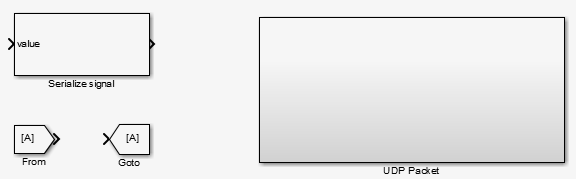
\includegraphics[width=.75\textwidth]{implementation/library}
	\caption{First implementation of the Monitoring System Library} 
	\label{fig:firstmonsys}
\end{figure}

\subsubsection{Signal Block}
The Signal Block consists of a pop-up and a Matlab function. In the pop-up, the parameters `Label', `Type', `Minimum Safe Value' and `Maximum Safe Value' can be defined by the user. The layout of this pop-up can be seen in figure \ref{fig:firstpopup}. The Matlab function takes these parameters and the signal value. The function then serializes them separately and merges the resulting arrays together. The code for serialization was adapted from Christian Kothe's implementation \cite{web:serialize}. The output of the block is the serialized array from the function.

\subsubsection{UDP Packet Subsystem}
The `UDP Packet' subsystem, shown in figure \ref{fig:firstmonsys}, needs to be copied over to the top level of the Simulink model it's being used in. The inside of this subsystem is shown in figure \ref{fig:firstudpsys}. As stated above, the From-block of each signal gets placed here. The serialized signals then get combined with a `Vector Concatenate' block into one big vector. The amount of inputs of this block can be changed, depending on how many signals need to be combined. Furthermore, a timer gets added at the beginning of the vector, so that it is possible to keep track of the elapsed time. This concatenated vector then gets send through to the `Send UDP packet' subsystem. This subsystem is being triggered with a rate of 50 Hz and sends out a UDP Packet at every trigger.

\begin{figure}[H]
	\centering
	\begin{minipage}{.39\textwidth}
		\centering
		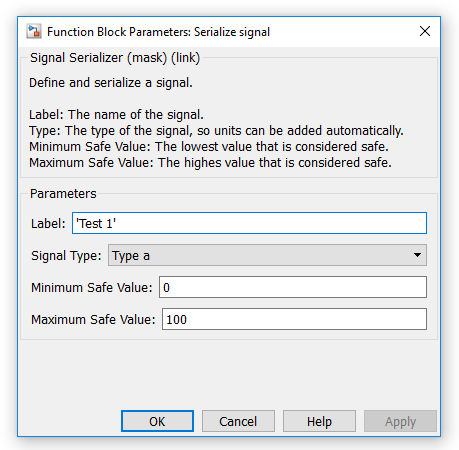
\includegraphics[width=\linewidth]{implementation/popup}
		\subcaption{Signal Block Pop-up}
		\label{fig:firstpopup}
	\end{minipage}
	\rulesep
	\begin{minipage}{.59\textwidth}
		\centering
		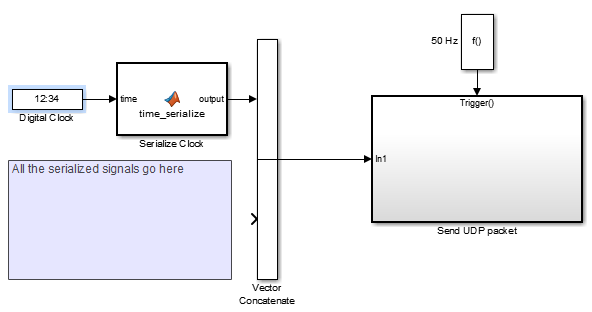
\includegraphics[width=\linewidth]{implementation/UDPPacket}
		\subcaption{UDP Packet Subsystem}
		\label{fig:firstudpsys}
	\end{minipage}
	\caption{More in-depth look at the blocks}
	\label{fig:firstimplementation}
\end{figure}

\subsubsection{Possible Improvements}
When the first implementation was completed, the exoskeleton was not completely assembled yet and did not have a Simulink model available. Therefore the team created a test simulation that used random values, instead of real signals. Once this was done, the team called the Tech Support of MathWorks, the makers of MATLAB and Simulink, to ask whether they knew more alternatives or ways to improve how the signal outputs were being transferred. After the Tech Support consulted among themselves, they replied that they too thought the Goto/From blocks-combination would be the best suited solution. They did give the suggestion to check whether it was possible to combine the signals in the subsystems instead, as this would reduce the amount of blocks in the `UDP Packet' Subsystem. The team would check whether it was possible to implement this in the final model.

\subsection{Final Implementation}\label{sec:simfinim}
As stated in the previous section, when the first version of the library was ready, the team had to wait before it could be tested in practice. In this section the changes to the first implementation will be described, that made sure the library worked with the exoskeleton model.



